\documentclass[spanish,a4paper, 11pt]{article}
\usepackage{anysize}
\papersize{29.7cm}{21cm} 
\usepackage[top=2.5cm, left=2.5cm, right=2.5cm, bottom=2.5cm]{geometry}

\usepackage{lmodern}
\usepackage[T1]{fontenc}
\usepackage[utf8x]{inputenc}
\usepackage[spanish,activeacute]{babel}

\usepackage{booktabs}
\usepackage{amssymb}
\usepackage{amsmath}
\usepackage{mathtools}
\usepackage{braket}
\usepackage{multirow}
\usepackage{titlesec}
\usepackage[font=small,labelfont=sf]{caption}
\usepackage{hyperref}
\usepackage{appendix}
\usepackage{soul}
\usepackage{framed}
\usepackage{fancyhdr}
\usepackage{graphicx}
\usepackage{caption}
\usepackage{subcaption}
\usepackage[lflt]{floatflt}
\usepackage{enumerate}
\usepackage{wrapfig}
\usepackage{float}
\usepackage{titlesec}
\usepackage{appendix}
\usepackage[xcolor]{mdframed}
\usepackage{titling}
\usepackage{enumitem}
\usepackage{chngpage}
\usepackage{algorithm}
\usepackage[noend]{algpseudocode}
\usepackage{natbib}
\usepackage{varwidth}

\renewcommand\spanishtablename{\textbf{Tabla}}
\renewcommand\spanishfigurename{\textbf{Figura}}
\algrenewcommand\algorithmicprocedure{\textbf{Procedimiento}}
\algrenewcommand\algorithmicdo{\textbf{haz}}
\algrenewcommand\algorithmicfor{\textbf{desde}}
\algrenewcommand\algorithmicif{\textbf{si}}
\algrenewcommand\algorithmicthen{\textbf{entonces}}
\algrenewcommand\algorithmicelse{\textbf{si no}}
\algrenewcommand\algorithmicwhile{\textbf{mientras que}}

\usepackage{tocloft}
\renewcommand{\cftsecleader}{\cftdotfill{\cftdotsep}}

\DeclareFontFamily{T1}{calligra}{}
\DeclareFontShape{T1}{calligra}{m}{n}{<->s*[1.44]callig15}{}
\DeclareMathAlphabet\mathcalligra   {T1}{calligra} {m} {n}
\DeclareMathAlphabet\mathzapf       {T1}{pzc} {mb} {it}
\DeclareMathAlphabet\mathchorus     {T1}{qzc} {m} {n}
\DeclareMathAlphabet\mathrsfso      {U}{rsfso}{m}{n}


\addto{\captionsspanish}{\renewcommand{\refname}{Bibliofgrafía}}

\graphicspath{{Figures/}}

\numberwithin{equation}{section}
\numberwithin{table}{section}
\numberwithin{figure}{section}

%\usepackage[
style = apa,
    backend=biber,
    bibstyle=numeric,
    citestyle=numeric-comp,
     maxcitenames=2,
    natbib=true,
    sorting = none,
    url=false, 
    doi=false,
    eprint=false
]{biblatex}
\addbibresource{Bibliografia.bib}
\DefineBibliographyStrings{spanish}{andothers = {et\addabbrvspace al\adddot}}

\pagestyle{fancy}
\fancyhf{}

\renewcommand{\headrulewidth}{0pt}

\author{Cabrera, Giovanni Alberto\\ gcbrera61@alumno.uned.es \and Gamazo, Ángel Javier \\ agamazo6@alumno.uned.es  \and Izaguirre, Gonzalo \\ gizaguirr2@alumno.uned.es }

\title{\textbf{Generación automática de datos etiquetados en imágen médica mediante el uso de GAN}\\ VISIÓN ARTIFICIAL \\ \textit{Máster Universitario en I.A. Avanzada}}
\date{Junio del 2019}
\fancyhead[L]{M2 Visión Artificial}
\fancyhead[R]{\rightmark}
\fancyfoot[R]{\thepage}
\captionsetup{width=\linewidth}

\begin{document}
\pagenumbering{gobble}
\maketitle
\vspace{1 cm}
\begin{figure}[H]
	\centering
	
\includegraphics[width=0.8\linewidth]{Logo.png}	
\end{figure}
\newpage

\pagenumbering{Roman}

\begin{abstract}
En los últimos años, la visión artificial ha evolucionado enormemente, en parte gracias a métodos basados en deep learning. Esta evolución se ha aprovechado en medicina, puesto que se han creado métodos capaces de detectar distintas lesiones en imágenes como magneto-resonancias o radiografías, de forma automática. Fruto de ello, se han creado también diversos concursos para encontrar el mejor método en multitud de disciplinas distintas, estando uno de ellos centrado en la segmentación de manchas de sustancia blanca en el cerebro, lo cual podría ayudar a prevenir enfermedades vasculares entre otras. En este trabajo, se pretende mejorar los resultados obtenidos por uno de los métodos presentados a dicho concurso, por medio de técnicas de aumento de datos.
\end{abstract}
	
	
	\renewcommand{\abstractname}{\textit{Abstract}}
	
\begin{abstract}
In the last years, artificial vision has evolved a lot, partly thanks to deep learning based methods. This evolution has benefited medicine, because there exist methods capable of detect several injuries by looking in images, such as MRI or X-ray, automatically. Besides, contests have been created to find the best method in different disciplines, being one of them focused on the segmentation of white matter hyperintensities, which could help to prevent vascular ills among others. In this work, the objective is to improve the results of one of the methods presented to that contests, using techniques of data augmentation.
\end{abstract}
\newpage
\tableofcontents
\newpage

\pagenumbering{arabic}
\setcounter{page}{3}
\section{Introducción}


En 2017, en las conferencias MICCAI (\textit{Medical Image Computing and Computer Assisted Intervention}), fue lanzado el concurso de Segmentación de Hiperintensidades de Materia Blanca (WMH). Este se trata de un concurso de análisis de imágenes médicas, en el que se pretende comparar directamente métodos para la segmentación automática de Hiperintensidades de Materia Blanca en el cerebro.\\
	
El interés en este campo radica en que estas hiperintensidades se encuentran comúnmente en personas mayores y están asociadas con varios desórdenes neurológicos y geriátricos, como problemas de humor o deterioro cognitivo.\\
	
Normalmente son encontradas en magneto-resonancias FLAIR y, aunque es posible marcar las zonas donde se encuentran las hiperintensidades a mano, es una tarea bastante laboriosa. Es por ello que técnicas basadas en la visión artificial y en aprendizaje máquina han ganado mucho peso en los últimos años, como una forma bastante prometedora para el diagnóstico automático de enfermedades.\\
	
En cuanto al concurso, desde la propia organización se proporciona un conjunto de entrenamiento que todos los participantes deben descargar y usarlo para desarrollar su propio método. El conjunto de test es guardado por la organización y no es hecho público en ningún momento, siendo únicamente utilizado para evaluar los distintos métodos. Para esta evaluación, además,  se han utlizado cinco métricas: coeficiente de similaridad de Dice, distancia de Hausdorff, diferencia absoluta de volumen, sensitividad para lesiones individuales y puntuación F1 para lesiones individuales.\\

Uno de los problemas más habituales y que limitan la precisión que pueden alcanzar los modelos basados en Deep Learning es la cantidad de información disponible. Conseguir una gran cantidad de datos etiquetados de imágenes médicas es normalmente una tarea demasiado costosa para ser llevada a cabo. Normalmente, para aumentar la cantidad de datos con los que una red es entrenada se realizan transformaciones aleatorias sobre las imágenes originales tales como rotaciones, inversiones o ligeros cambios en el contraste. Sin embargo, el enfoque dado en este trabajo es radicalmente diferente. El modelo inicialmente propuesto por \citet{Goodfellow2014}, \textbf{G}enerative \textbf{A}dversarial \textbf{N}etwork (GAN) provee de un método atractivo para obtener un modelo generativo que sea capaz de crear nuevas imágenes. Estas redes se componen de dos subredes: un \textit{generador} y un \textit{discriminador} que son enfrentadas. El generador genera imágenes a partir de un vector de ruido. El discriminador es una red normal de clasificación que recibe datos reales y datos generados por el generador. Su objetivo es clasificar las imágenes en reales o generadas. El objetivo del generador es engañar lo máximo posible al discriminador. Este tipo de redes han sido utilizadas de forma satisfactoria en generación de imágenes \\cite{Ishaan2017}.\\

En este trabajo nos centraremos en el estudio de técnicas de aumentado de datos en tareas de segmentación, implementando un sistema generador de imágenes etiquetadas que resolvería el problema de la anotación manual y que podría dar lugar a redes neuronales mucho más efectivas en tareas de segmentación debido a que serían entrenadas con una mayor cantidad de imágenes a pesar de tener un número limitado de imágenes anotadas por médicos.\\

A pesar de que el objetivo central del trabajo era mejorar el funcionamiento del modelo ganador del campeonato de segmentación de WMH, en este trabajo nos centramos únicamente en el modelo generativo de imágenes. Las causas de este hecho se resumen en dos. En primer lugar, la estructura del modelo del que se parte (U-Net) está hecho de forma que se entrena la red con todos los datos menos los de un paciente, así para todos los pacientes. En este caso, vamos a generar imágenes artificiales que no pertenecen a ningún paciente, por lo que sería necesaria una reestructuración del método de entrenamiento del modelo y consideramos que este sería objeto de un futuro trabajo. En segundo lugar, para reentrenar el modelo de la U-Net se requiere de una capacidad de cómputo de la que en este momento no disponemos.\\

El trabajo se estructura en varias secciones. En la Sección \ref{RedesNeur} se realiza una introducción al deep learning y a las redes neuronales, en la Sección \ref{Implementacion} se explica el modelo concreto utilizado en este trabajo y los frameworks utilizados en su implementación. Por último, en las Secciones \ref{Resultados} y \ref{Discusion} se muestran y analizan los resultados obtenidos y su posible contribución al área de la imagen médica.

\newpage
\section{Redes Neuronales}
\label{RedesNeur}

En los últimos años, gracias al significativo aumento de la capacidad de cómputo de los procesadores y tarjetas gráficas de los últimos años, las redes neuronales han sido utilizadas para reconocer objetos en imágenes en tiempo real \cite{Redmon2015}, analizar voces de forma automática \cite{Hinton2012} o traducción de texto \cite{Vinyals2014}. El aspecto clave del Deep Learning es el aprendizaje automático de representaciones significativas y de la estructura interna de un conjunto de datos de entrada. Esto se consigue utilizando una gran cantidad de capas que procesan la información. Estas capas calculan, en base a unos parámetros ajustables (pesos), una función de salida diferenciable que depende de los parámetros de entrada. A mayor número de capas existentes, más abstracta será la representación a la que se llegue. En clasificación de imágenes puede verse cómo las primeras capas detectan estructuras sencillas como bordes en la imagen, mientras que las capas más profundas detectan estructuras más complejas.\\

A pesar de que el Deep Learning se ha utilizado de forma satisfactoria en numerosos campos, nosotros nos centramos en su aplicación en el campo de la visión artificial, en concreto en la segmentación de imágenes. Este problema consiste, por ejemplo, en detectar objetos dentro de una imagen o, aplicado en medicina, la detección en una imagen de una determinada estructura de interés.

\subsection{Neuronas artificiales}

Las neuronas artificiales son la estructura fundamental de las redes neuronales. Una neurona artificial es una función matemática concebida como un modelo de las neuronas biológicas. Una neurona recibe una serie de entradas $x_1, \hdots, x_N$ , las suma de forma ponderada utilizando unos pesos $w_1, \hdots, w_N$ a la que se añade un término $b$ de \textit{bias} y, utilizando una función de activación, genera una determinada salida. La función de activación suele ser una función no lineal, de forma que la neurona sea no lineal La salida de una neurona puede calcularse como
\begin{equation}
s = \sigma \left( \sum_i x_i \cdot w_i + b_i \right) = \sigma (z),
\end{equation}
dondeque puede expresarse más convenientemente utilizando notación vectorial, de forma que obtenemos.
\begin{equation}
s = \sigma(x^T \cdot w + b) = \sigma(z)
\end{equation}

En la Figura \ref{Neurona} se muestra de forma gráfica la estructura y funcionamiento de una neurona artificial.

\begin{figure}[H]
	\centering
	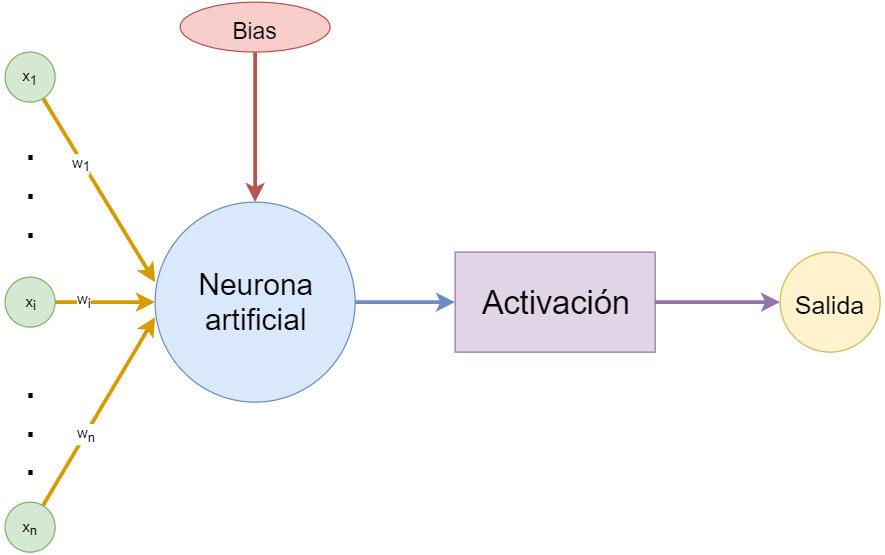
\includegraphics[width=0.6\linewidth]{Neurona.png}
	\caption{Estructura de una neurona artificial.}
	\label{Neurona}	
\end{figure}

A pesar de ser un modelo relativamente simple, tiene el potencial para ser utilizado en problemas de muy diversa índole. Si se toma como activación la función
\begin{equation}
\sigma(z) = \frac{1}{1+e^{-z}},
\end{equation}
(función sigmoide), la neurona puede ser utilizada para problemas de clasificación binaria, mientras que con otras funciones, las neuronas pueden usarse para otras tareas.

\subsection{Redes Neuronales \textit{Feed-Forward}}

Inicialmente se crearon modelos denominados perceptrones, que utilizaban una única neurona modelada como se ha descrito anteriormente. Sin embargo, las redes neuronales son mucho más potentes si combinamos varias neuronas. En la Figura \ref{FNN} puede verse un ejemplo de este tipo de redes. La red consiste en una capa de entrada, en la que se tienen los datos con los que se entrenará la red, una capa oculta en la que cada neurona está conectada a todas las entradas y una capa de salida con una única neurona que genera una salida. La deonminación de Deep Learning viene del gran número de capas ocultas que se suelen utilizar en modelos complejos.

\begin{figure}[H]
	\centering
	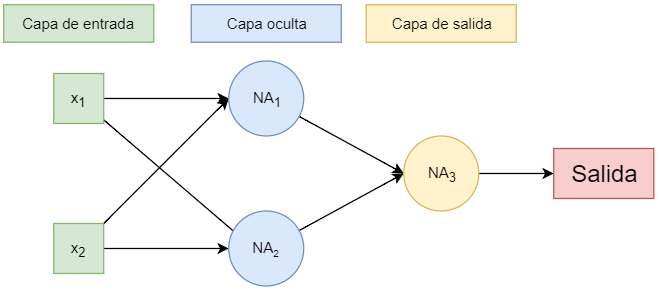
\includegraphics[width=0.7\linewidth]{FNN.png}
	\caption{Estructura de una red neuronal feed-forward. Cada una de las neuronas (NA) tiene la estructura de la Figura \ref{Neurona}.}
	\label{FNN}	
\end{figure}

\subsection{Funciones de activación}

Como hemos mencionado, una parte fundamental de las neuronas artificiales (y el origen de su potencial, puesto que introducen la no linealidad en el modelo) es la función de activación. Esta función se aplica sobre el resultado de la suma pesada de las entradas de la neurona. En esta sección detallamos las funciones de activación más utilizadas.

\subsubsection{Sigmoide}

Esta función se define matemáticamente como
\begin{equation}
\sigma(x) = \frac{1}{1+e^{-x}},
\end{equation}
Que tiene como dominio de entrada cualquier numero $x \in \mathbb{R}$ y como conjunto imagen el intervalo $(0,1)$. Esta función tiene un origen biológico, dado que mapea cualquier valor de entrada a un rango de estados que pueden interpretarse como si la neurona se dispara o no. Tiene la ventaja de ser diferenciable, con 
\begin{equation}
\sigma^\prime(x) = \sigma(x)  \cdot \left(1- \sigma(x) \right) .
\end{equation}
Esta función suele utilizarse cuando la salida de una neurona se ha de interpretar como una función de probabilidad. Sin embargo, esta función tiene la desventaja de que se satura rápido. Es decir, hay un amplio rango de valores para los que la salida de la función es prácticamente la misma (numeros alejados de 0), resultando en que su gradiente será muy cercano a 0, lo cual supondrá, como se verá más adelante, un problema.

\subsubsection{Rectified Linear Unit (ReLU)}

La función ReLU se define como
\begin{equation}
ReLU(x) = \max{(0,x)}.
\end{equation}

En la Figura \ref{ReLU} se muestra esta función gráficamente. Tiene como ventajas la no saturación en su parte positiva y su facilidad de cómputo, ya que simplemente se ha de umbralizar la salida y además su derivada siempre es 1 o 0.

\begin{figure}[H]
	\centering
	\includegraphics[width=0.7\linewidth]{ReLU.png}
	\caption{Representación gráfica de la función ReLU.}
	\label{ReLU}	
\end{figure}

Uno de los principales problemas es la parte plana de la función ReLU. A pesar de tener la ventaja de tener una derivada constante en su parte positiva, la derivada nula en la parte negativa puede ser una desventaja, como veremos.

\subsubsection{Leaky ReLU}

La función se define como 
\begin{equation}
LeakyReLU(x) = \begin{cases}
\alpha x & x < 0,\\
x & x \geq 0
\end{cases},
\end{equation}
donde $\alpha$ es un parámetro $ 0 < \alpha \ll 1$, de forma que evitamos el problema de la derivada nula de la función para $x<0$.
\subsection{Optimización de redes neuronales}

Hasta el momento hemos visto la estructura de una red neuronal básica. Sin embargo, se ha explicado el proceso de entrenamiento de una red neuronal. Si la salida de la red es la pertenencia o no de un registro a una clase, es de esperar que mediante una inicialización aleatoria se obtengan buenos resultados. La parte ajustable de una red neuronal son los pesos de las conexiones entre neuronas. En el caso de la Figura \ref{FNN} únicamente son 5 pesos, pero en redes muy grandes este número puede ascender a varios millones.\\

Por tanto, el proceso de entrenamiento de una red es el proceso mediante el cual, partiendo de unos pesos inicializados al azar, ajustamos los pesos de las conexiones entre neuronas de forma que el resultado sea el deseado. Métodos de entrenamiento de redes neuronales hay de muchos tipos y consideramos que explicarlos queda fuera del alcance del trabajo. La mayoría de algoritmos de entrenamiento se basan en la definición de una función de error que hay que optimizar. A grandes rasgos, se calcula la derivada de la función de error respecto de cada peso y se ajusta el peso de acuerdo al valor de esta derivada. Uno de los métodos de optimización más utilizados en la actualizad, propuesto por \citep{Kingma2014} es el denominado ADAM.

\subsection{U-Net}

El método base a utilizar, descrito más en detalle en el artículo  \citep{Li2018}, ha sido el ganador de este concurso, y se basa en el uso de una variante de redes convolucionales llamada U-Net.\\
	
Así, su arquitectura toma como entrada los cortes axiales de dos modalidades de escáneres de magneto-resonancia, T1 y FLAIR, las cuales son juntadas como entrada de dos canales. En la imagen inferior se puede observar dicha arquitectura.

	\begin{figure}[H]
	\centering
		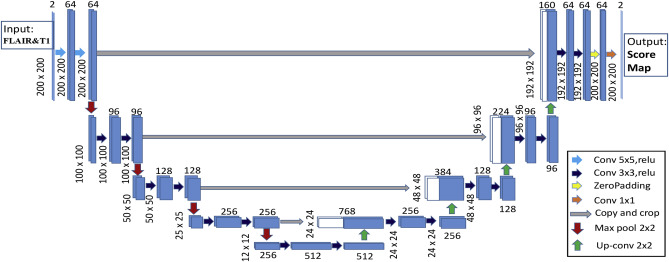
\includegraphics[width=\linewidth]{img1.jpg}
		\caption[\textit{Arquitectura del modelo}]{Arquitectura del modelo}
		\label{fig:FCC}
	\end{figure}

En este modelo, dos capas convolucionales son usadas de forma repetida, cada una seguida por una unidad de rectificado lineal (ReLU) y una operación max-pooling de 2 x 2 con paso 2. En la capa final, una convolución de 1 x 1 es utilizada para mapear cada vector de características de 64 componentes en dos clases. En total, se utilizan 19 capas convolucionales. \\

Como función de pérdida se utiliza la pérdida de Dice, la cual es formulada de la siguiente forma:
	
	\begin{figure}[H]
	 	\centering
		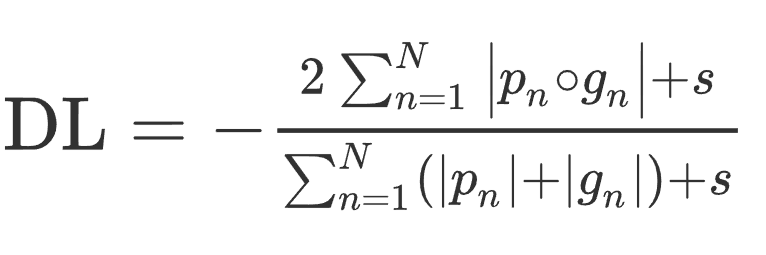
\includegraphics[height=2cm]{dice_loss.png}
		\label{fig:Dice}
	\end{figure}
	
	
donde G=\{g$_{1}$, .... g$_{N}$\} es la probabilidad observable de segmentación sobre N capas, y P=\{p$_{1}$, ..., p$_{N}'$\} la probabilidad predicha sobre N capas.\\
	
Por último, cabe mencionar que este método, como su nombre indica, utiliza técnicas de conjuntos, las cuales son útiles para reducir los problemas de exceso asociados a las redes neuronales. Estas combinan múltiples modelos de aprendizaje para obtener mejor rendimiento a la hora de predecir.	


\section{GAN: Generative Adversial Networks}
	
	
Para la realización de este proyecto, se ha decidido a utilizar redes GAN para conseguir un aumento de datos considerables, y que así el modelo descrito anteriormente pueda obtener mejores resultados. Por tanto, resulta conveniente en un primer momento, explicar el concepto de estas redes.\\
	
Las GAN, del inglés \textit{Generative Adversial Networks}, traducido al español como Red Generativa Antagónica, son un framework para estimar modelos generativos. Consisten en dos submodelos claramente diferenciables, típicamente implementados como redes neuronales: El generador \textit{G} y el discriminador \textit{D}.\\
	
El funcionamiento de estas redes es sencillo. Por un lado, el generador es entrenado para generar imágenes $G(z)$ las cuales se parezcan a la distribución de los datos de entrenamiento $p_{R}$, utilizando un vector de ruido latente $z$, muestreado a partir de la distribución $p_{z}$; mientras que el discriminador recibe tanto imágenes generadas como el conjunto de datos de entrenamiento real $x$, y es entrenado para diferenciarlas.\\
	
De este modo, el generador es entrenado para minimizar la posibilidad de que el discriminador rechaze las imágenes generadas $(D(G(z)) \supset 0)$, mientras que el discriminador es entrenado para maximizar la probabilidad de acertar $(D(G(z)) \supset 0), (D(x) \supset 1)$. Esto lleva a la siguiente función minimax:
	
\begin{figure}[H]
	 \centering
	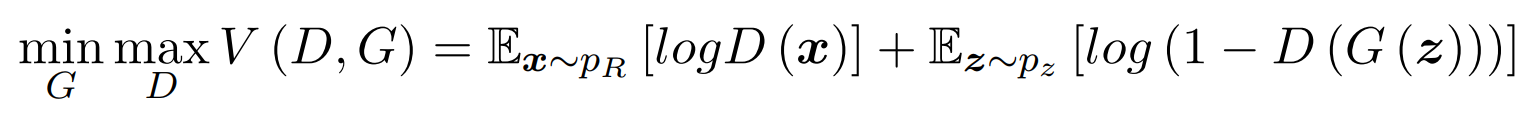
\includegraphics[height=1cm]{minimax.png}
	\label{fig:minimax}
\end{figure}
	
	
	A continuación se muestra un ejemplo de la arquitectura típica de una GAN:
	
\begin{figure}[H]
 	\centering
	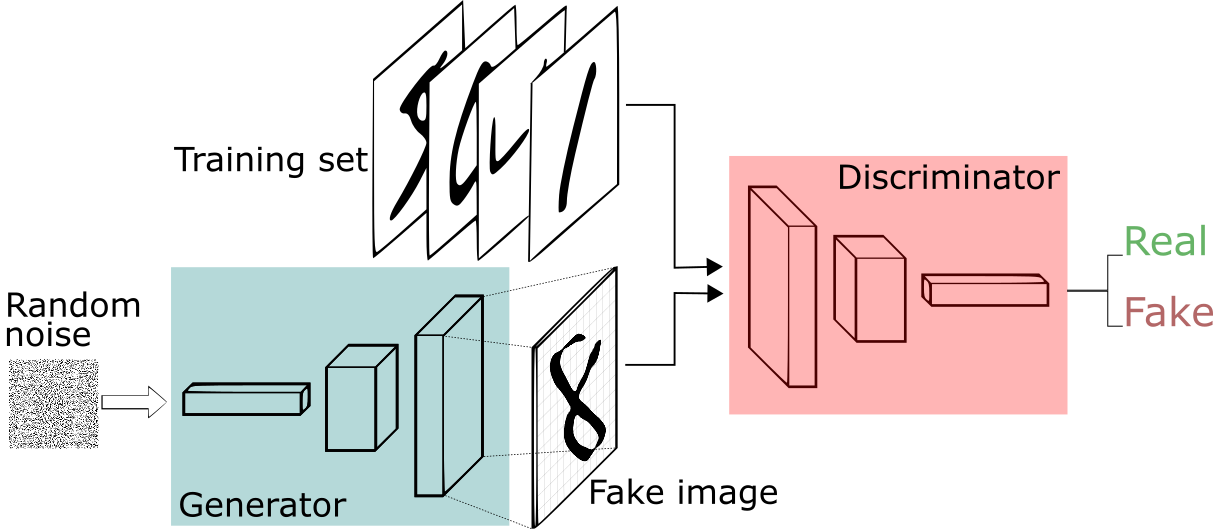
\includegraphics[width=\linewidth]{gan.png}
	\label{fig:gan}
\end{figure}	
	
	
Este tipo de redes son bastante recientes, y están siendo ampliamente investigadas. Fruto de esas investigaciones, son nuevos tipos de GAN, como las DCGAN (\textit{Deep Convolutional Generative Adversial Network}), las cuales tratan de incorporar los métodos más recientemente creados para las redes convolucionales.\\
	
También se encuentran las WGAN (\textit{Wasserstein Generative Adversial Network}), cuya principal motivación es analizar las distintas formas de medir la distancia entre la distribución del modelo \textit{p$_{G}$}, y la distribución real \textit{p$_{R}$}. Originalmente, las formulación de las GAN mostraba que la función objetivo para optimizar es la divergencia de \textit{Jensen-Shannon}. Sin embargo, para las WGAN, es utilizada la función de distancia \textit{Earth-Mover}, o distancia \textit{Wasserstein-1}, la cual intuitivamente calcula el coste del plan óptimo para transformar la distribución \textit{p$_{R}$} en \textit{p$_{G}$}. A continuación se especifica la fórmula:
	
\begin{figure}[H]
 	\centering
	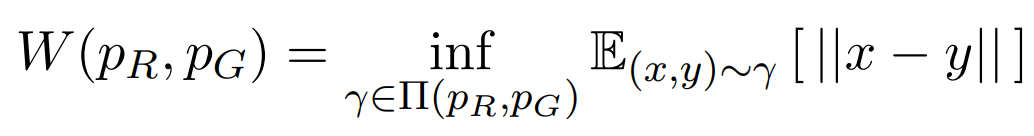
\includegraphics[height=1cm]{wasserstein.png}
	\label{fig:wasserstein}
\end{figure}	
	
	
Dentro de las WGAN, también se pueden encontran las WGAN-GP (\textit{Wasserstein Generative Adversial Networks with Gradient Penalty}), las cuales surgieron como respuesta a que algunas configuraciones de las WGAN guiaban a muestras de baja calidad o completa falta de convergencia.
	
\begin{figure}[H]
	\centering
	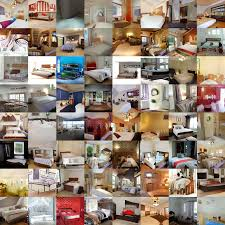
\includegraphics[width=6cm]{lsun.jpg}
	\label{fig:lsun_bedroom}
	\caption{Muestras creadas por una WGAN-GP entrenada en el conjunto de entrenamiento de habitaciones LSUN.}
\end{figure}	
\newpage
	
\section{Implementación}
\label{Implementacion}

\newpage

	
\section{Resultados}
\label{Resultados}	

	
\newpage
\section{Discusión}
\label{Discusion}
	
	
\section{Conclusiones}
	
\newpage
	
%\hypersetup{allcolors=black}
%%\nocite{*}
%\newpage
%\thispagestyle{empty}
%\addcontentsline{toc}{section}{Bibliografía}
%\printbibliography[title = Bibliografía]}
\end{document}
